% Options for packages loaded elsewhere
\PassOptionsToPackage{unicode}{hyperref}
\PassOptionsToPackage{hyphens}{url}
% !TeX program = pdfLaTeX
\documentclass[12pt]{article}
\usepackage{amsmath}
\usepackage{graphicx,psfrag,epsf}
\usepackage{enumerate}
\usepackage{textcomp}


%\pdfminorversion=4
% NOTE: To produce blinded version, replace "0" with "1" below.
\newcommand{\blind}{0}

% DON'T change margins - should be 1 inch all around.
\addtolength{\oddsidemargin}{-.5in}%
\addtolength{\evensidemargin}{-1in}%
\addtolength{\textwidth}{1in}%
\addtolength{\textheight}{1.7in}%
\addtolength{\topmargin}{-1in}%

%% load any required packages here



% tightlist command for lists without linebreak
\providecommand{\tightlist}{%
  \setlength{\itemsep}{0pt}\setlength{\parskip}{0pt}}

% From pandoc table feature
\usepackage{longtable,booktabs,array}
\usepackage{calc} % for calculating minipage widths
% Correct order of tables after \paragraph or \subparagraph
\usepackage{etoolbox}
\makeatletter
\patchcmd\longtable{\par}{\if@noskipsec\mbox{}\fi\par}{}{}
\makeatother
% Allow footnotes in longtable head/foot
\IfFileExists{footnotehyper.sty}{\usepackage{footnotehyper}}{\usepackage{footnote}}
\makesavenoteenv{longtable}

% Pandoc citation processing
\newlength{\cslhangindent}
\setlength{\cslhangindent}{1.5em}
\newlength{\csllabelwidth}
\setlength{\csllabelwidth}{3em}
\newlength{\cslentryspacingunit} % times entry-spacing
\setlength{\cslentryspacingunit}{\parskip}
% for Pandoc 2.8 to 2.10.1
\newenvironment{cslreferences}%
  {}%
  {\par}
% For Pandoc 2.11+
\newenvironment{CSLReferences}[2] % #1 hanging-ident, #2 entry spacing
 {% don't indent paragraphs
  \setlength{\parindent}{0pt}
  % turn on hanging indent if param 1 is 1
  \ifodd #1
  \let\oldpar\par
  \def\par{\hangindent=\cslhangindent\oldpar}
  \fi
  % set entry spacing
  \setlength{\parskip}{#2\cslentryspacingunit}
 }%
 {}
\usepackage{calc}
\newcommand{\CSLBlock}[1]{#1\hfill\break}
\newcommand{\CSLLeftMargin}[1]{\parbox[t]{\csllabelwidth}{#1}}
\newcommand{\CSLRightInline}[1]{\parbox[t]{\linewidth - \csllabelwidth}{#1}\break}
\newcommand{\CSLIndent}[1]{\hspace{\cslhangindent}#1}

\usepackage{amsmath}
\usepackage{subfig}

\IfFileExists{bookmark.sty}{\usepackage{bookmark}}{\usepackage{hyperref}}
\IfFileExists{xurl.sty}{\usepackage{xurl}}{} % add URL line breaks if available
\hypersetup{
  pdftitle={Supplementary Material for ``Bayesian Detection of Bias in Peremptory Challenges Using Historical Strike Data''},
  hidelinks,
  pdfcreator={LaTeX via pandoc}}



\begin{document}


\def\spacingset#1{\renewcommand{\baselinestretch}%
{#1}\small\normalsize} \spacingset{1}


%%%%%%%%%%%%%%%%%%%%%%%%%%%%%%%%%%%%%%%%%%%%%%%%%%%%%%%%%%%%%%%%%%%%%%%%%%%%%%

\if0\blind
{
  \title{\bf Supplementary Material for ``Bayesian Detection of Bias in Peremptory Challenges Using Historical Strike Data''}

  \author{
        \href{https://orcid.org/0000-0001-7387-1307}{Sachin S. Pandya} \\
    University of Connecticut\\
     and \\     Xiaomeng Li \\
    University of Connecticut\\
     and \\     \href{https://orcid.org/0000-0003-1934-1932}{Eric Barón} \\
    University of Connecticut\\
     and \\     \href{https://orcid.org/0000-0002-9576-0517}{Timothy E. Moore} \\
    University of Connecticut\\
      }
  \maketitle
} \fi

\if1\blind
{
  \bigskip
  \bigskip
  \bigskip
  \begin{center}
    {\LARGE\bf Supplementary Material for ``Bayesian Detection of Bias in Peremptory Challenges Using Historical Strike Data''}
  \end{center}
  \medskip
} \fi

\bigskip

\noindent%
 

\vfill

\newpage
\spacingset{1.9} % DON'T change the spacing!

Here, we extend section 3 of the paper by reporting our simulation results for 90\% and 80\% credible intervals. We also extend the discussion in section 3.2 of the paper by discussing data collection and presenting additional illustrations of how a lawyer might use the prototype app.

\hypertarget{bias-detection-with-90-and-80-credible-intervals}{%
\subsection{Bias Detection with 90\% and 80\% Credible Intervals}\label{bias-detection-with-90-and-80-credible-intervals}}

The choice of credible interval can affect bias detection as we define it, because the larger the credible interval one chooses, the greater the chance that zero falls within it, and vice-versa. Here, we report simulation results for bias detection for 90\% intervals for trials with fifteen, ten, and six strikes per side (Figures \ref{fig:figbd9015}, \ref{fig:figbd9010}, and \ref{fig:figbd906}, respectively), and the same for 80\% credible intervals (Figures \ref{fig:figbd8015}, \ref{fig:figbd8010}, and \ref{fig:figbd806}).

\begin{figure}

{\centering 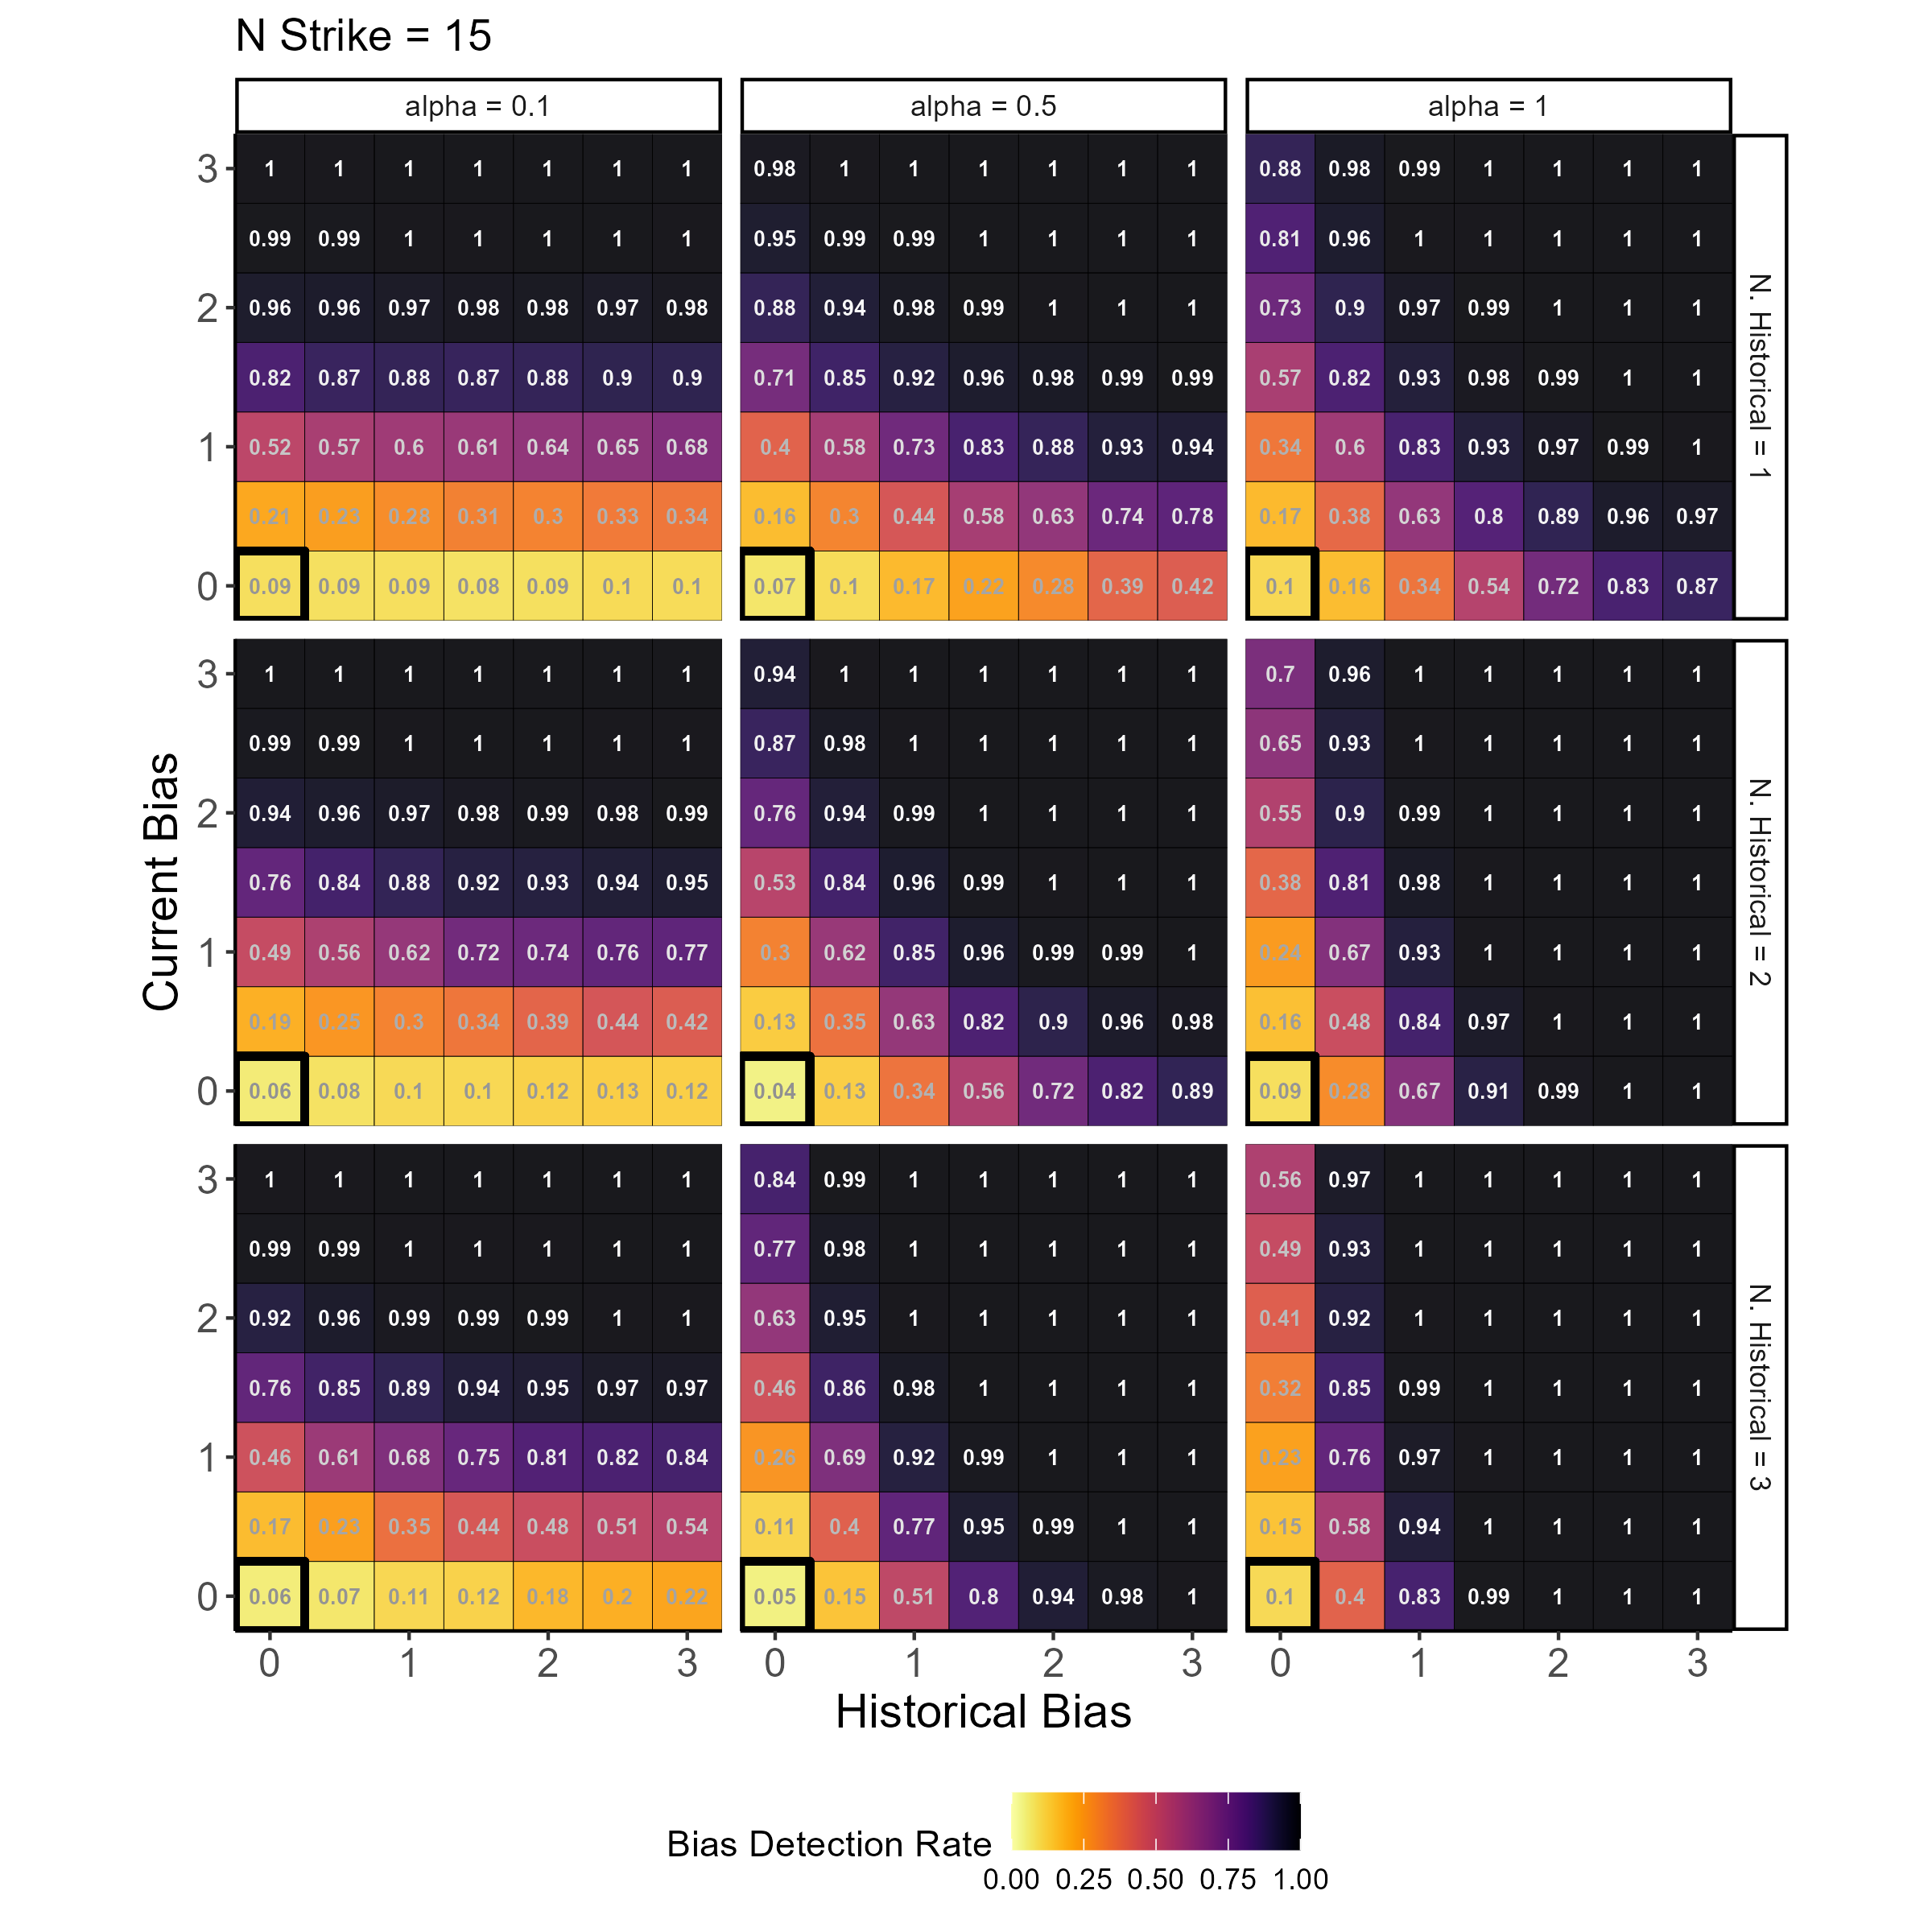
\includegraphics[width=0.95\linewidth]{../figures/pp15_90CI} 

}

\caption{Bias Detection Rates, 90 pct credible interval, 15 strike scenario}\label{fig:figbd9015}
\end{figure}

\begin{figure}

{\centering 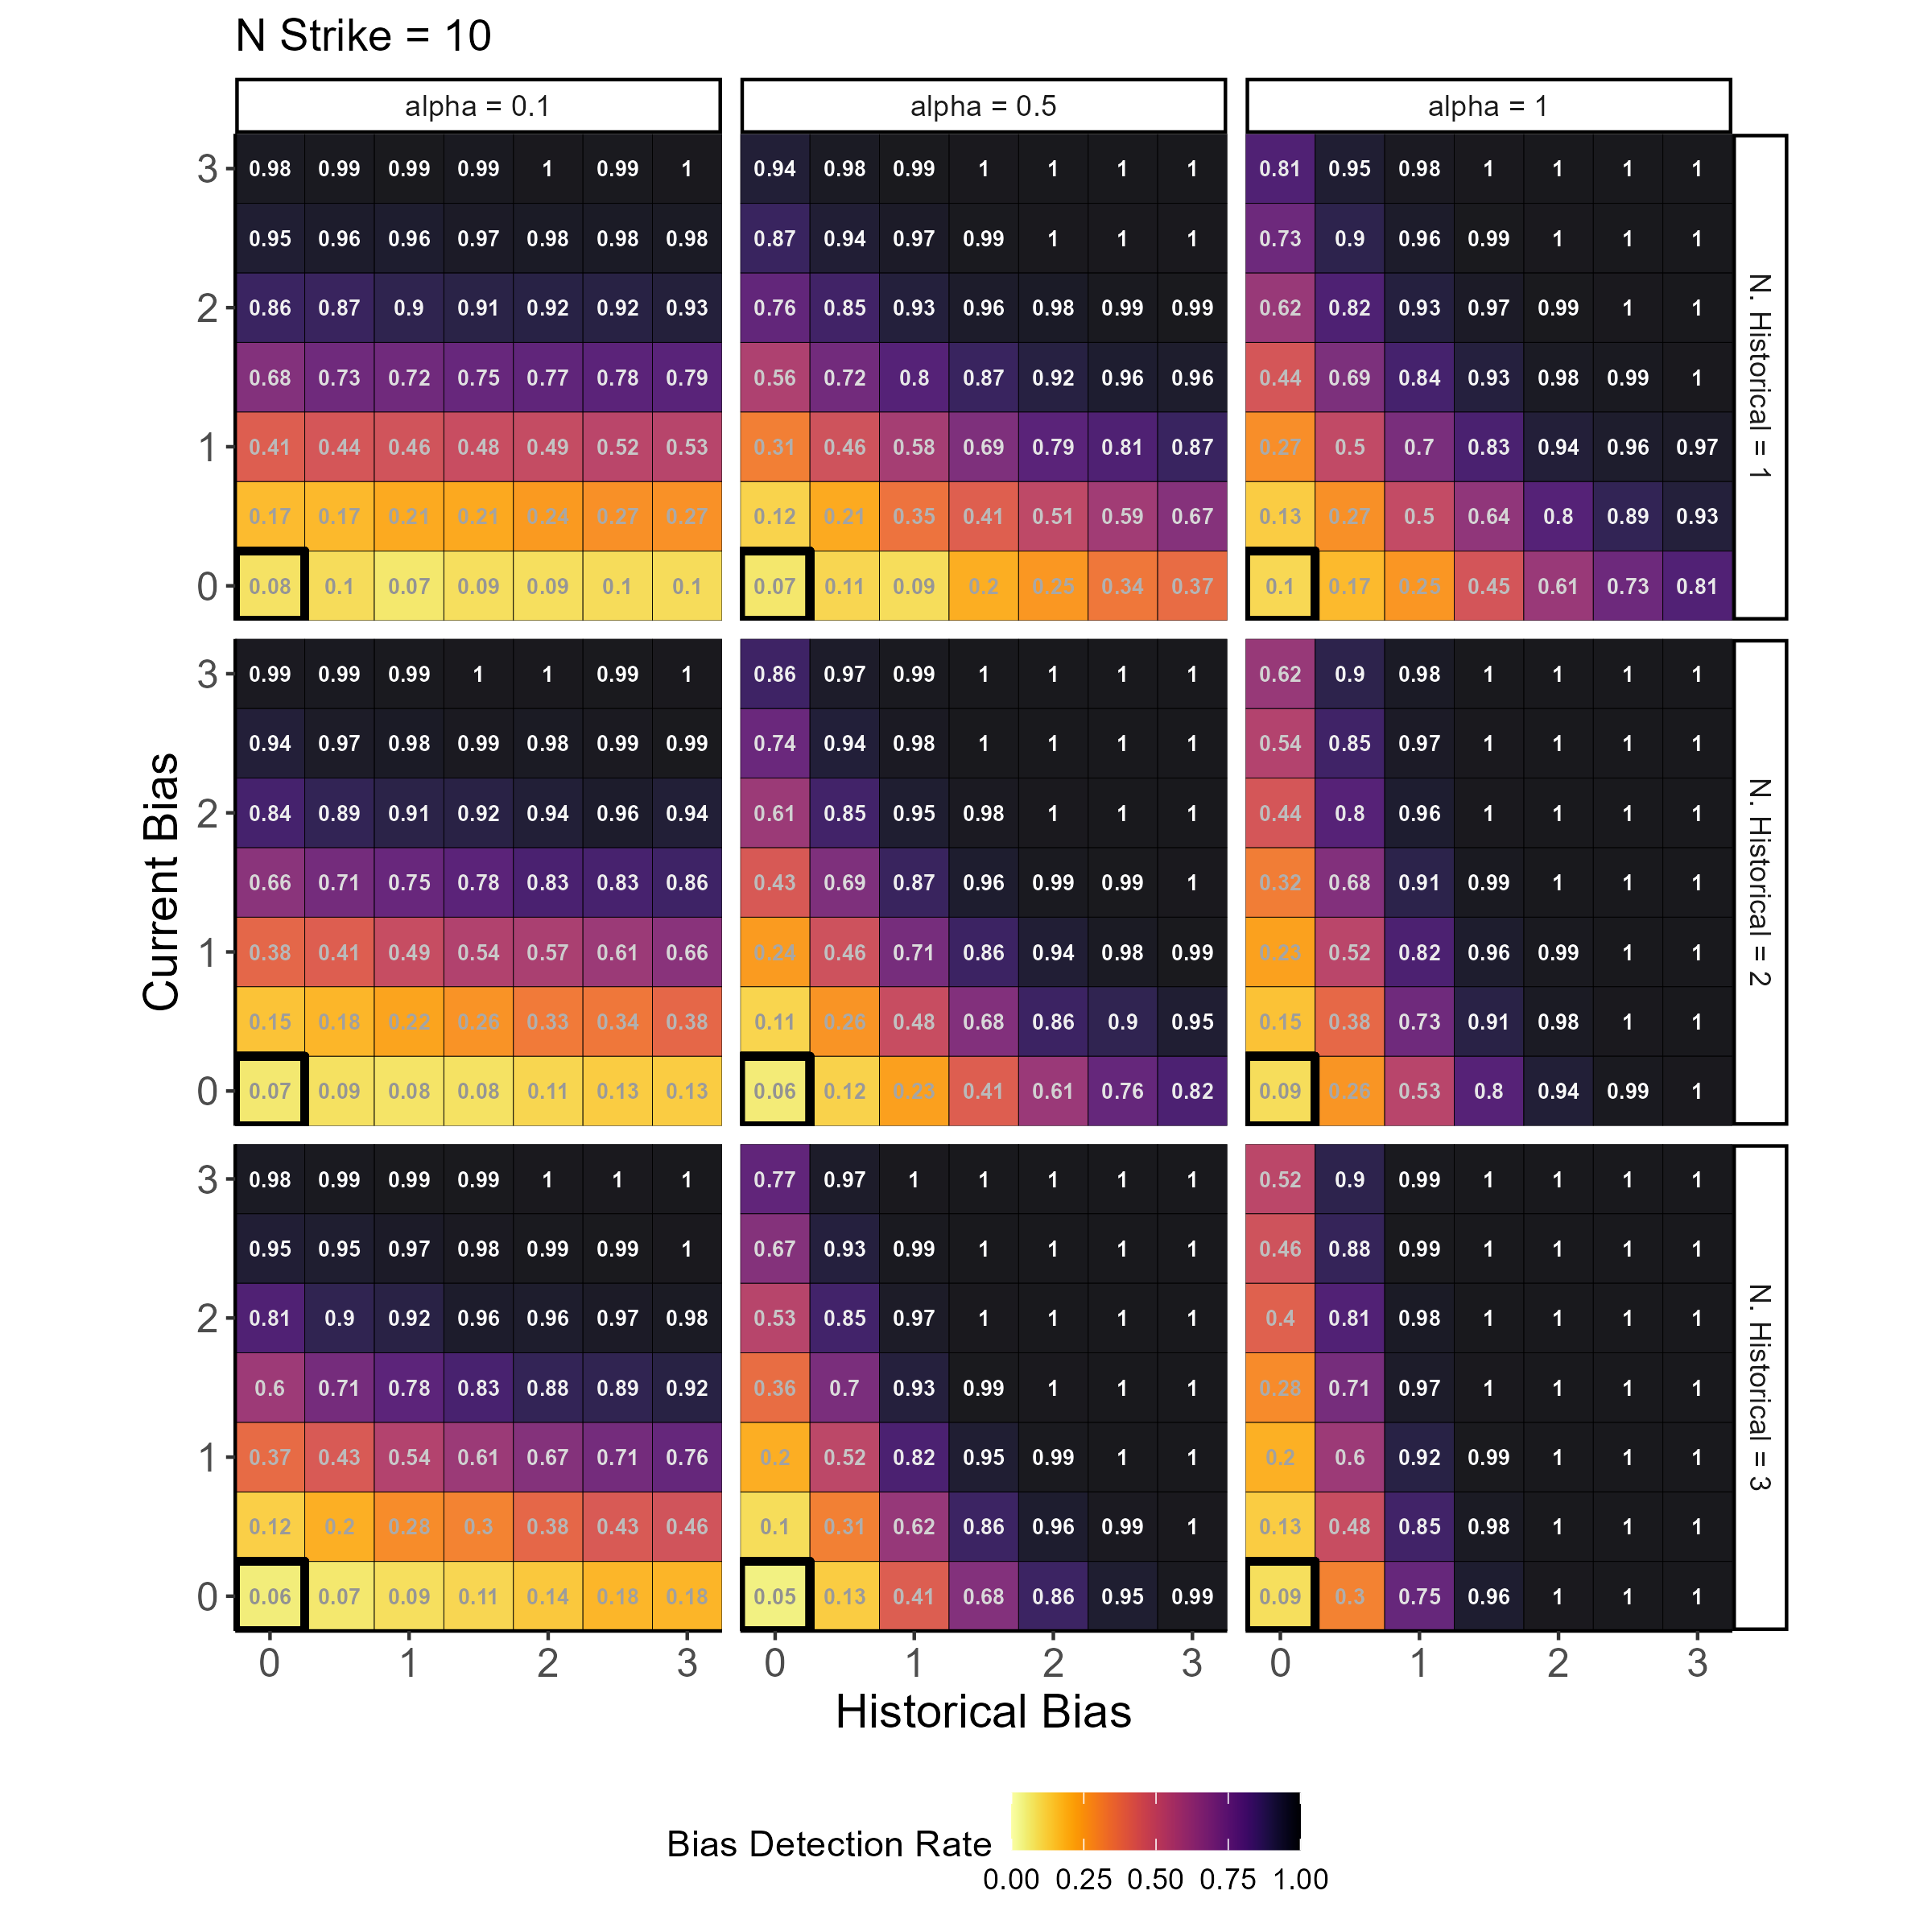
\includegraphics[width=0.95\linewidth]{../figures/pp10_90CI} 

}

\caption{Bias Detection Rates (90 pct credible interval, 10 strikes scenario)}\label{fig:figbd9010}
\end{figure}

\begin{figure}

{\centering 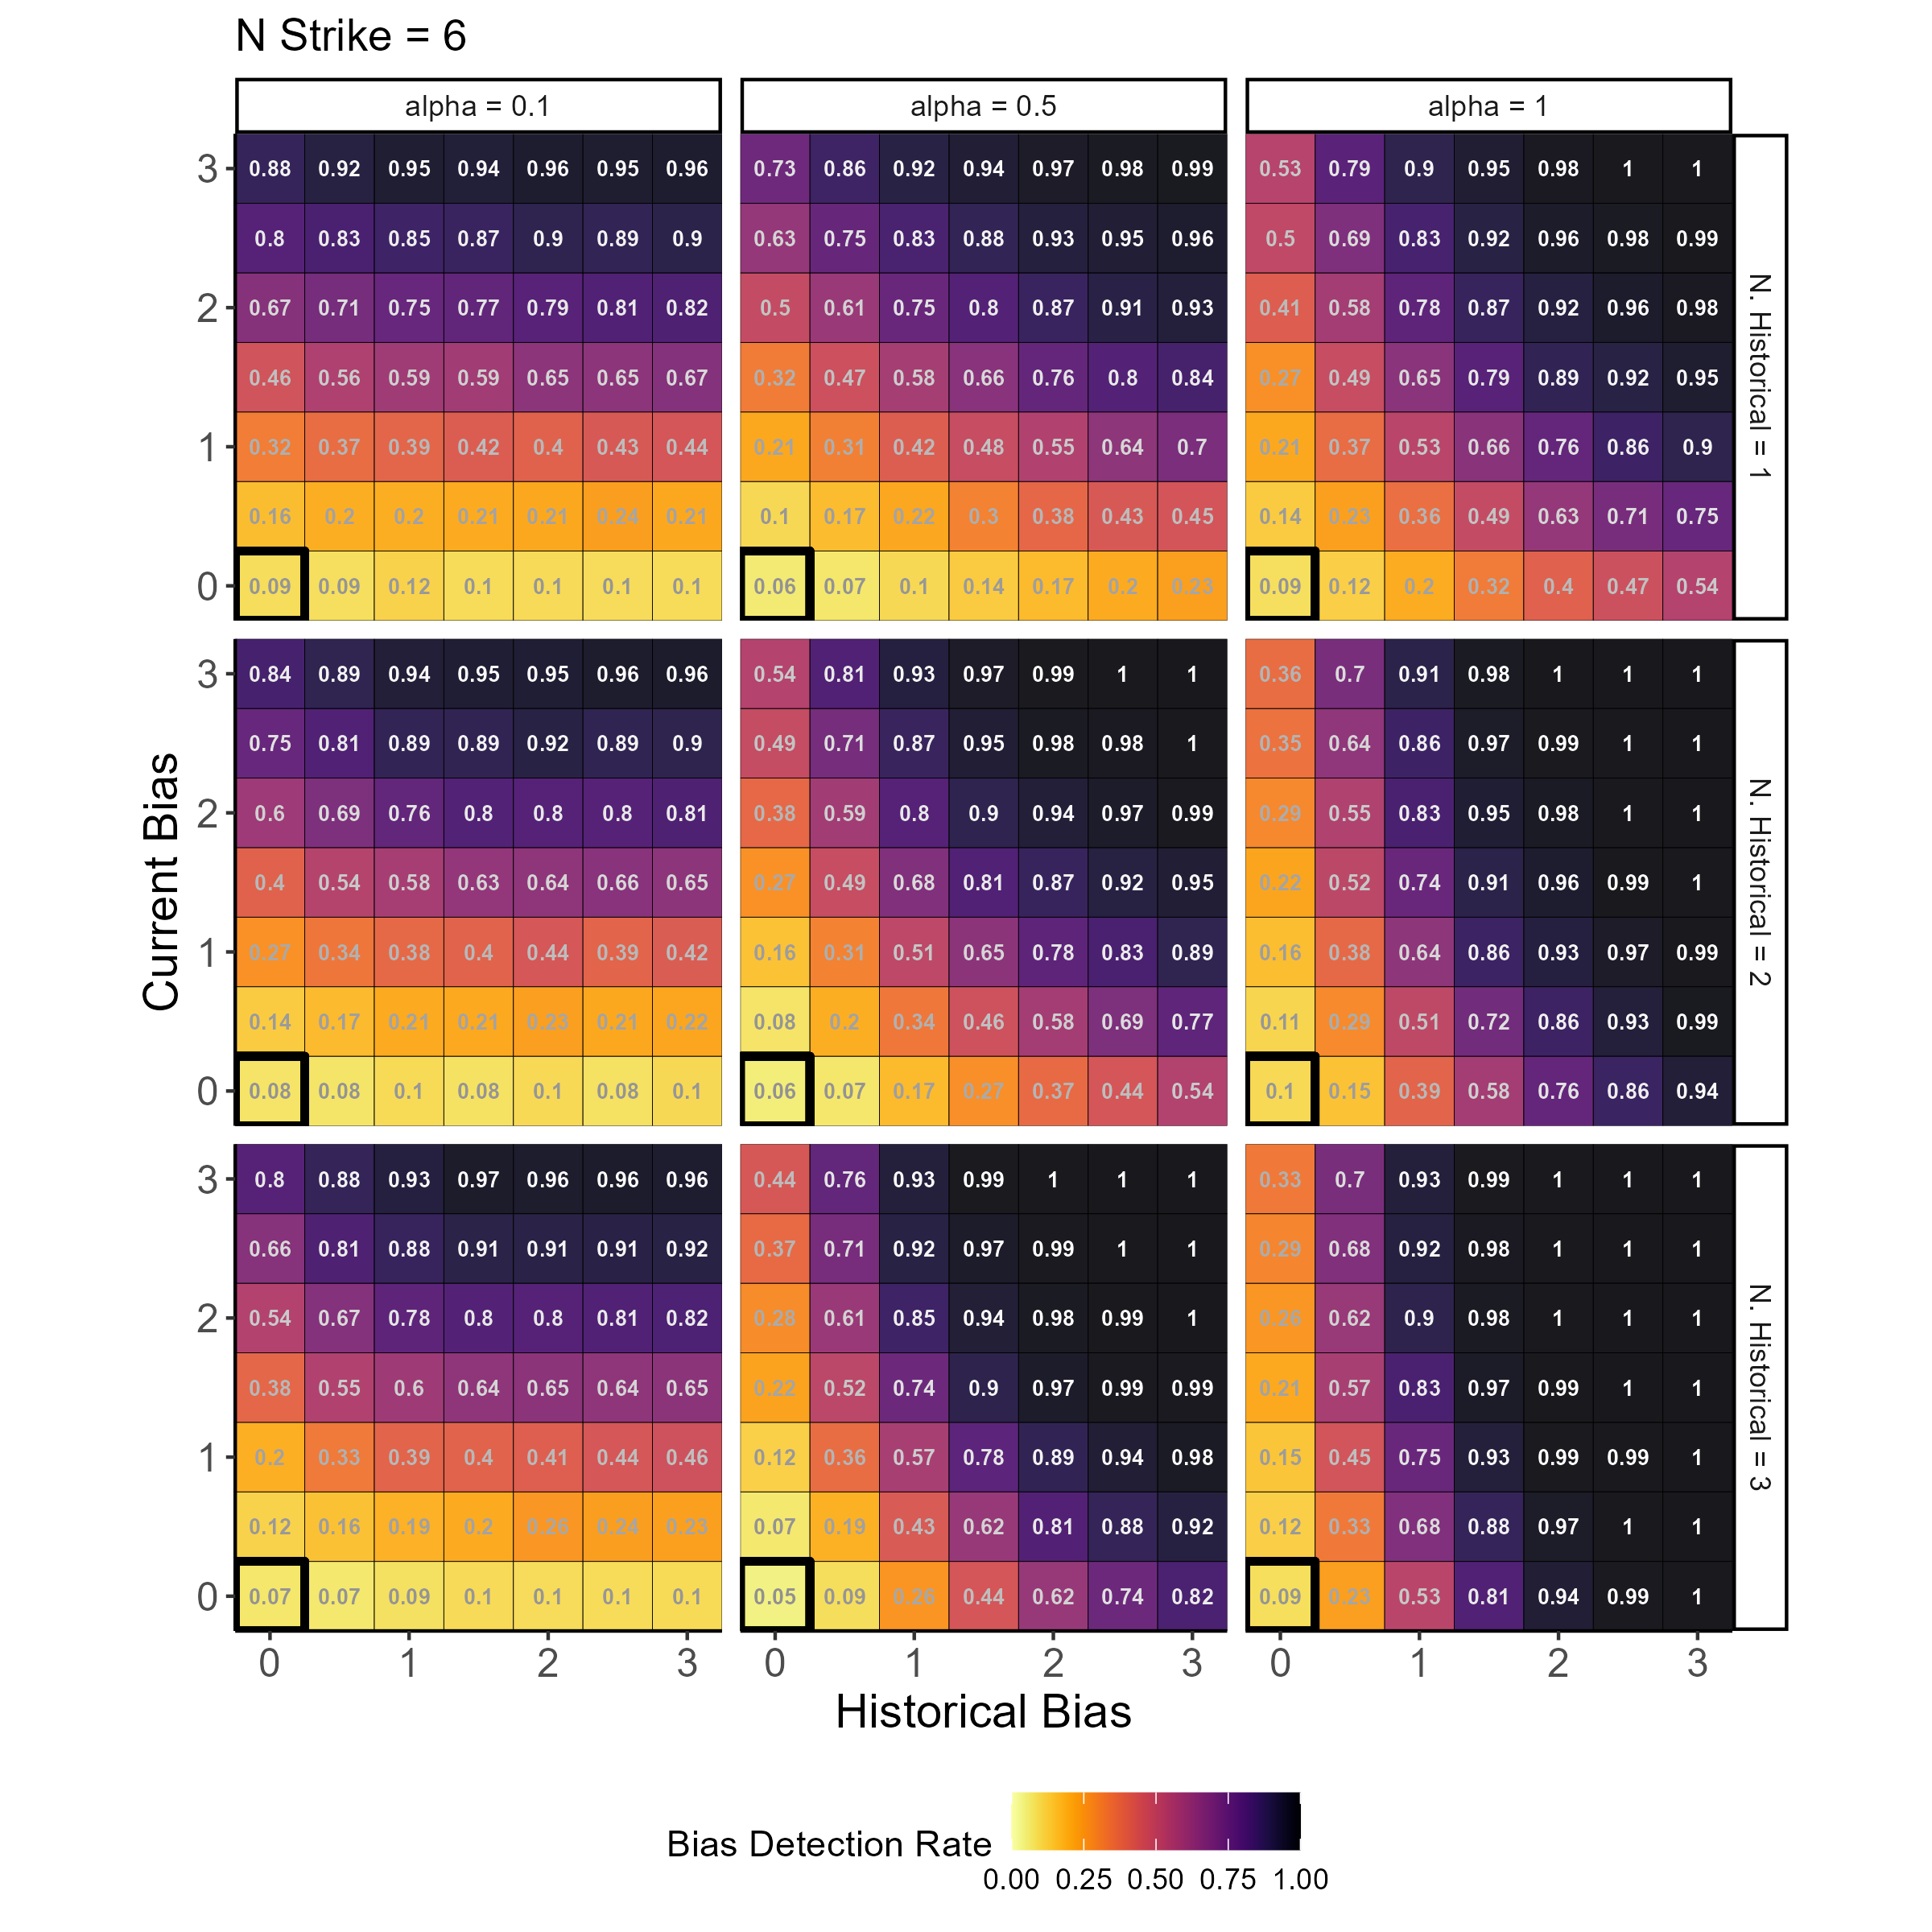
\includegraphics[width=0.95\linewidth]{../figures/pp6_90CI} 

}

\caption{Bias Detection Rates based on 90 pct credible interval for 6 strike scenario}\label{fig:figbd906}
\end{figure}

\begin{figure}

{\centering 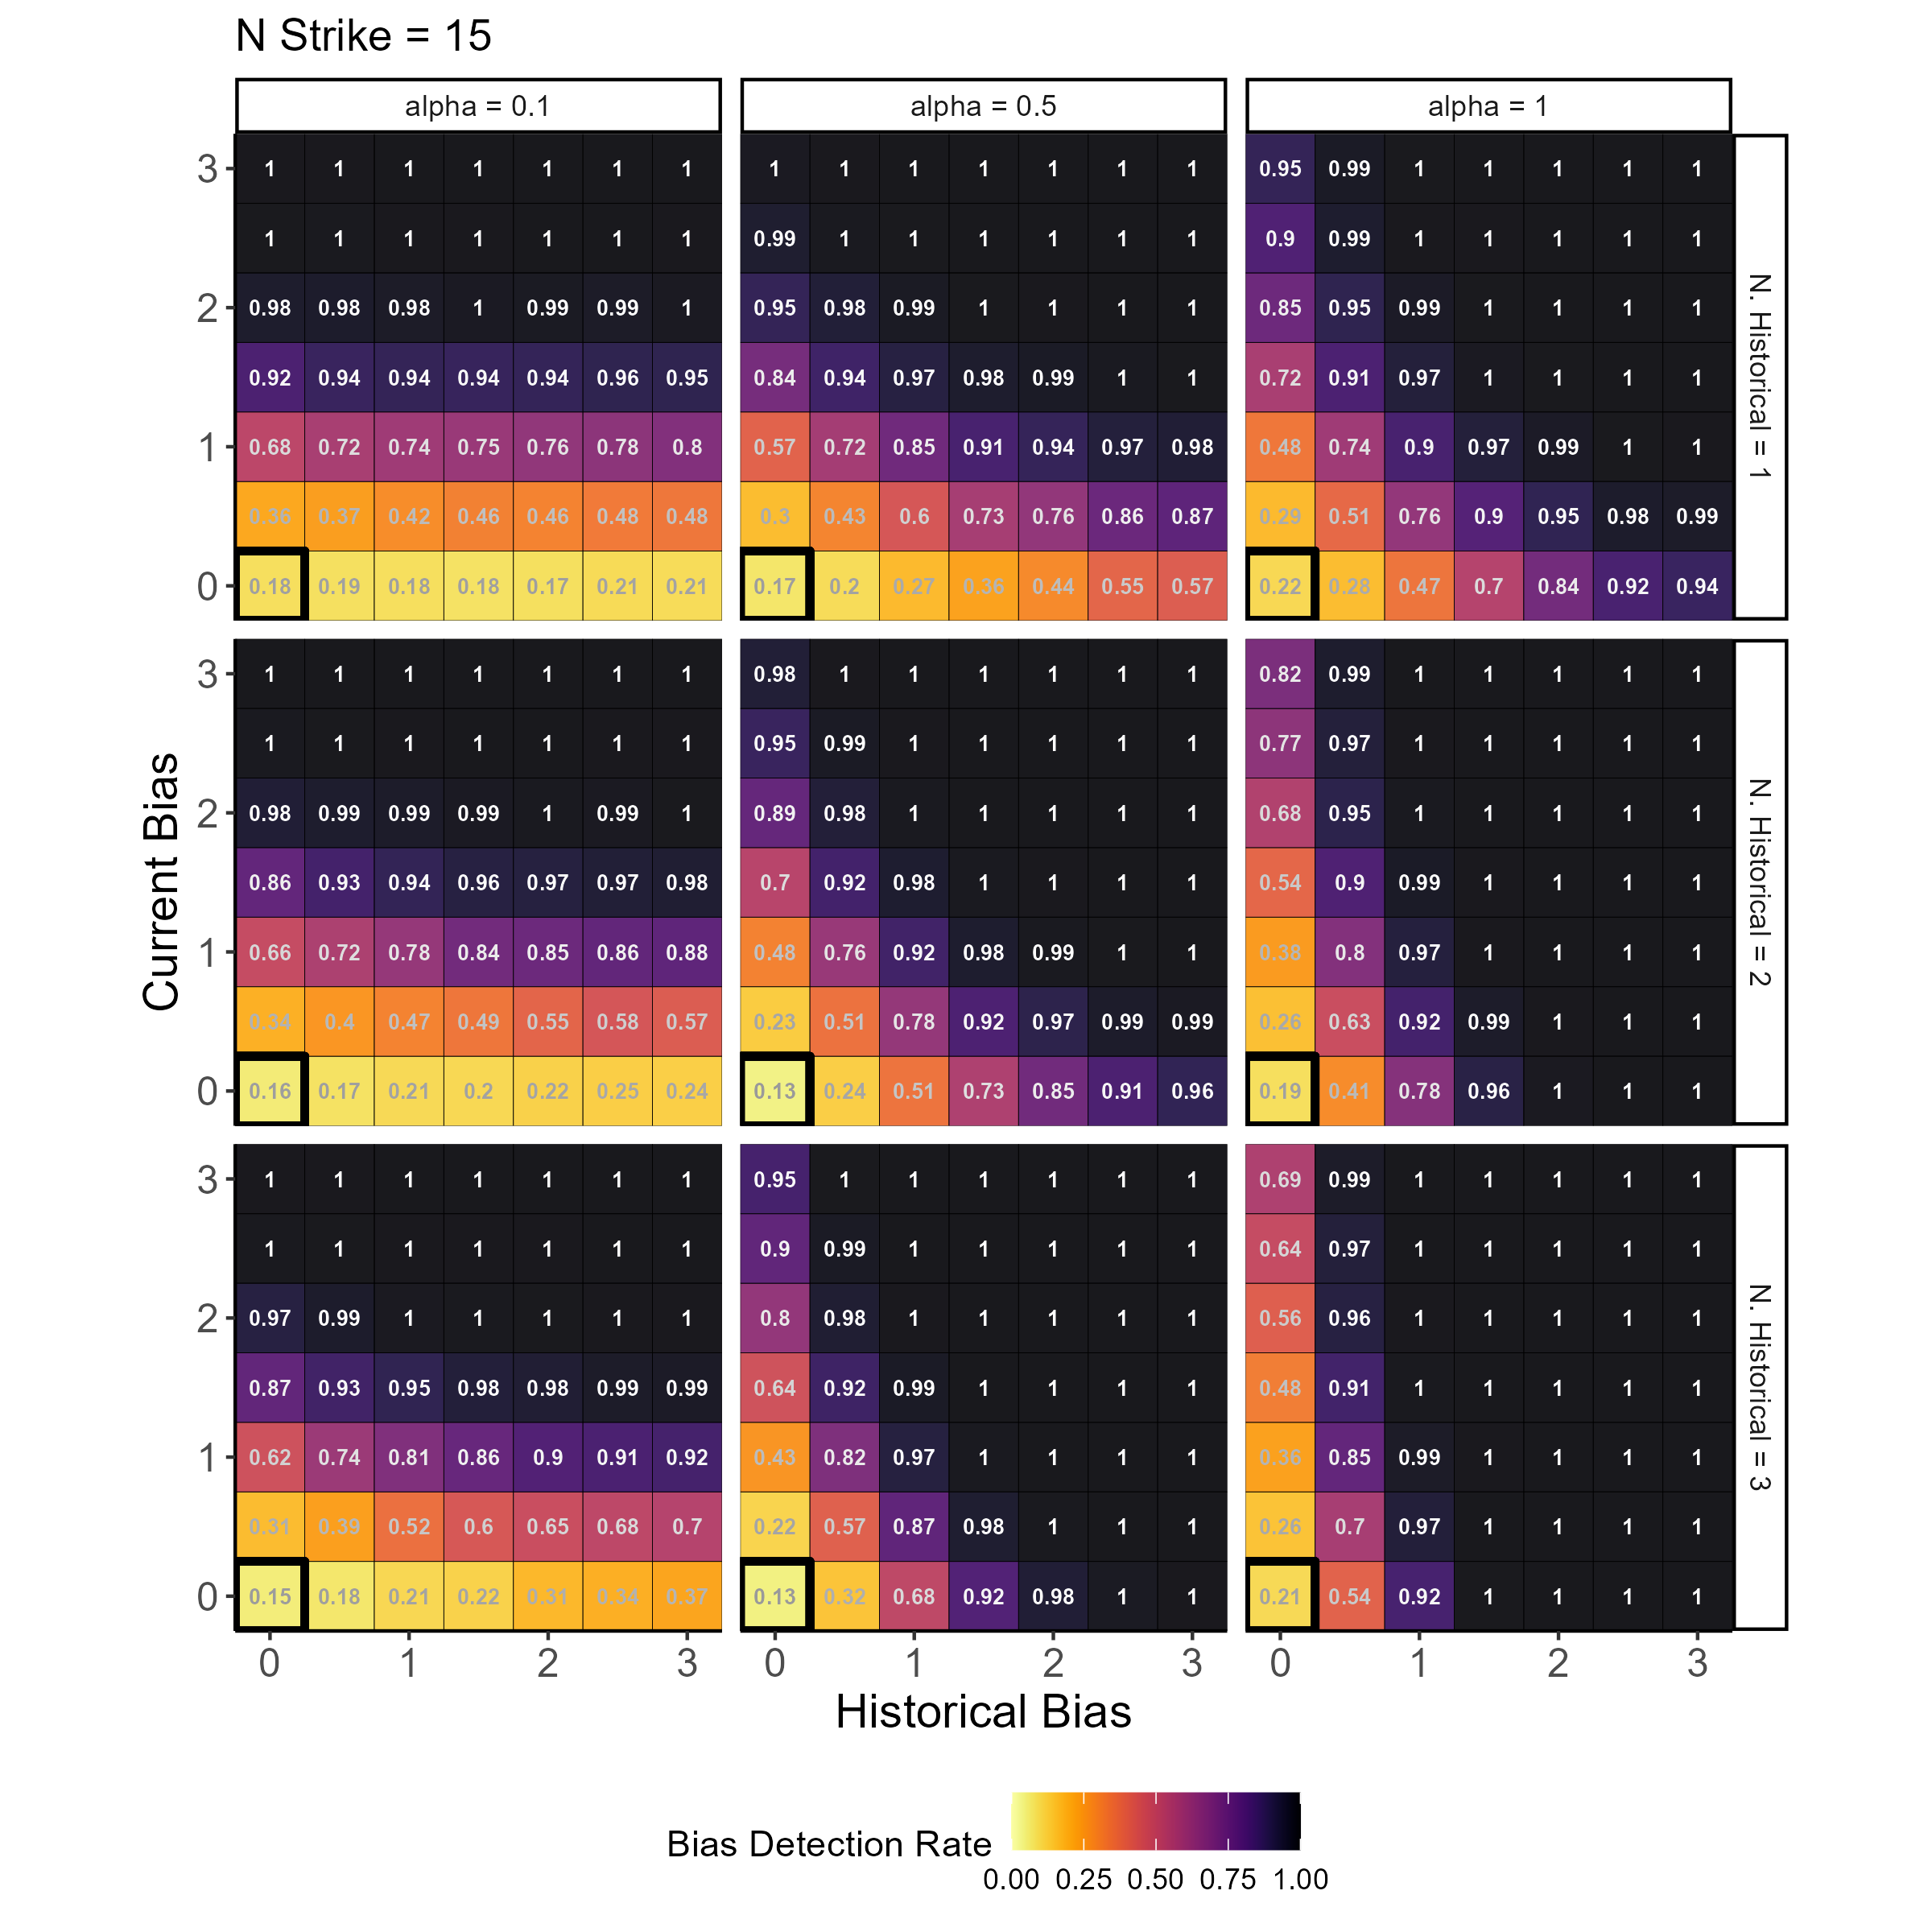
\includegraphics[width=0.95\linewidth]{../figures/pp15_80CI} 

}

\caption{Bias Detection Rates, 80 pct credible interval, 15 strike scenario}\label{fig:figbd8015}
\end{figure}

\begin{figure}

{\centering 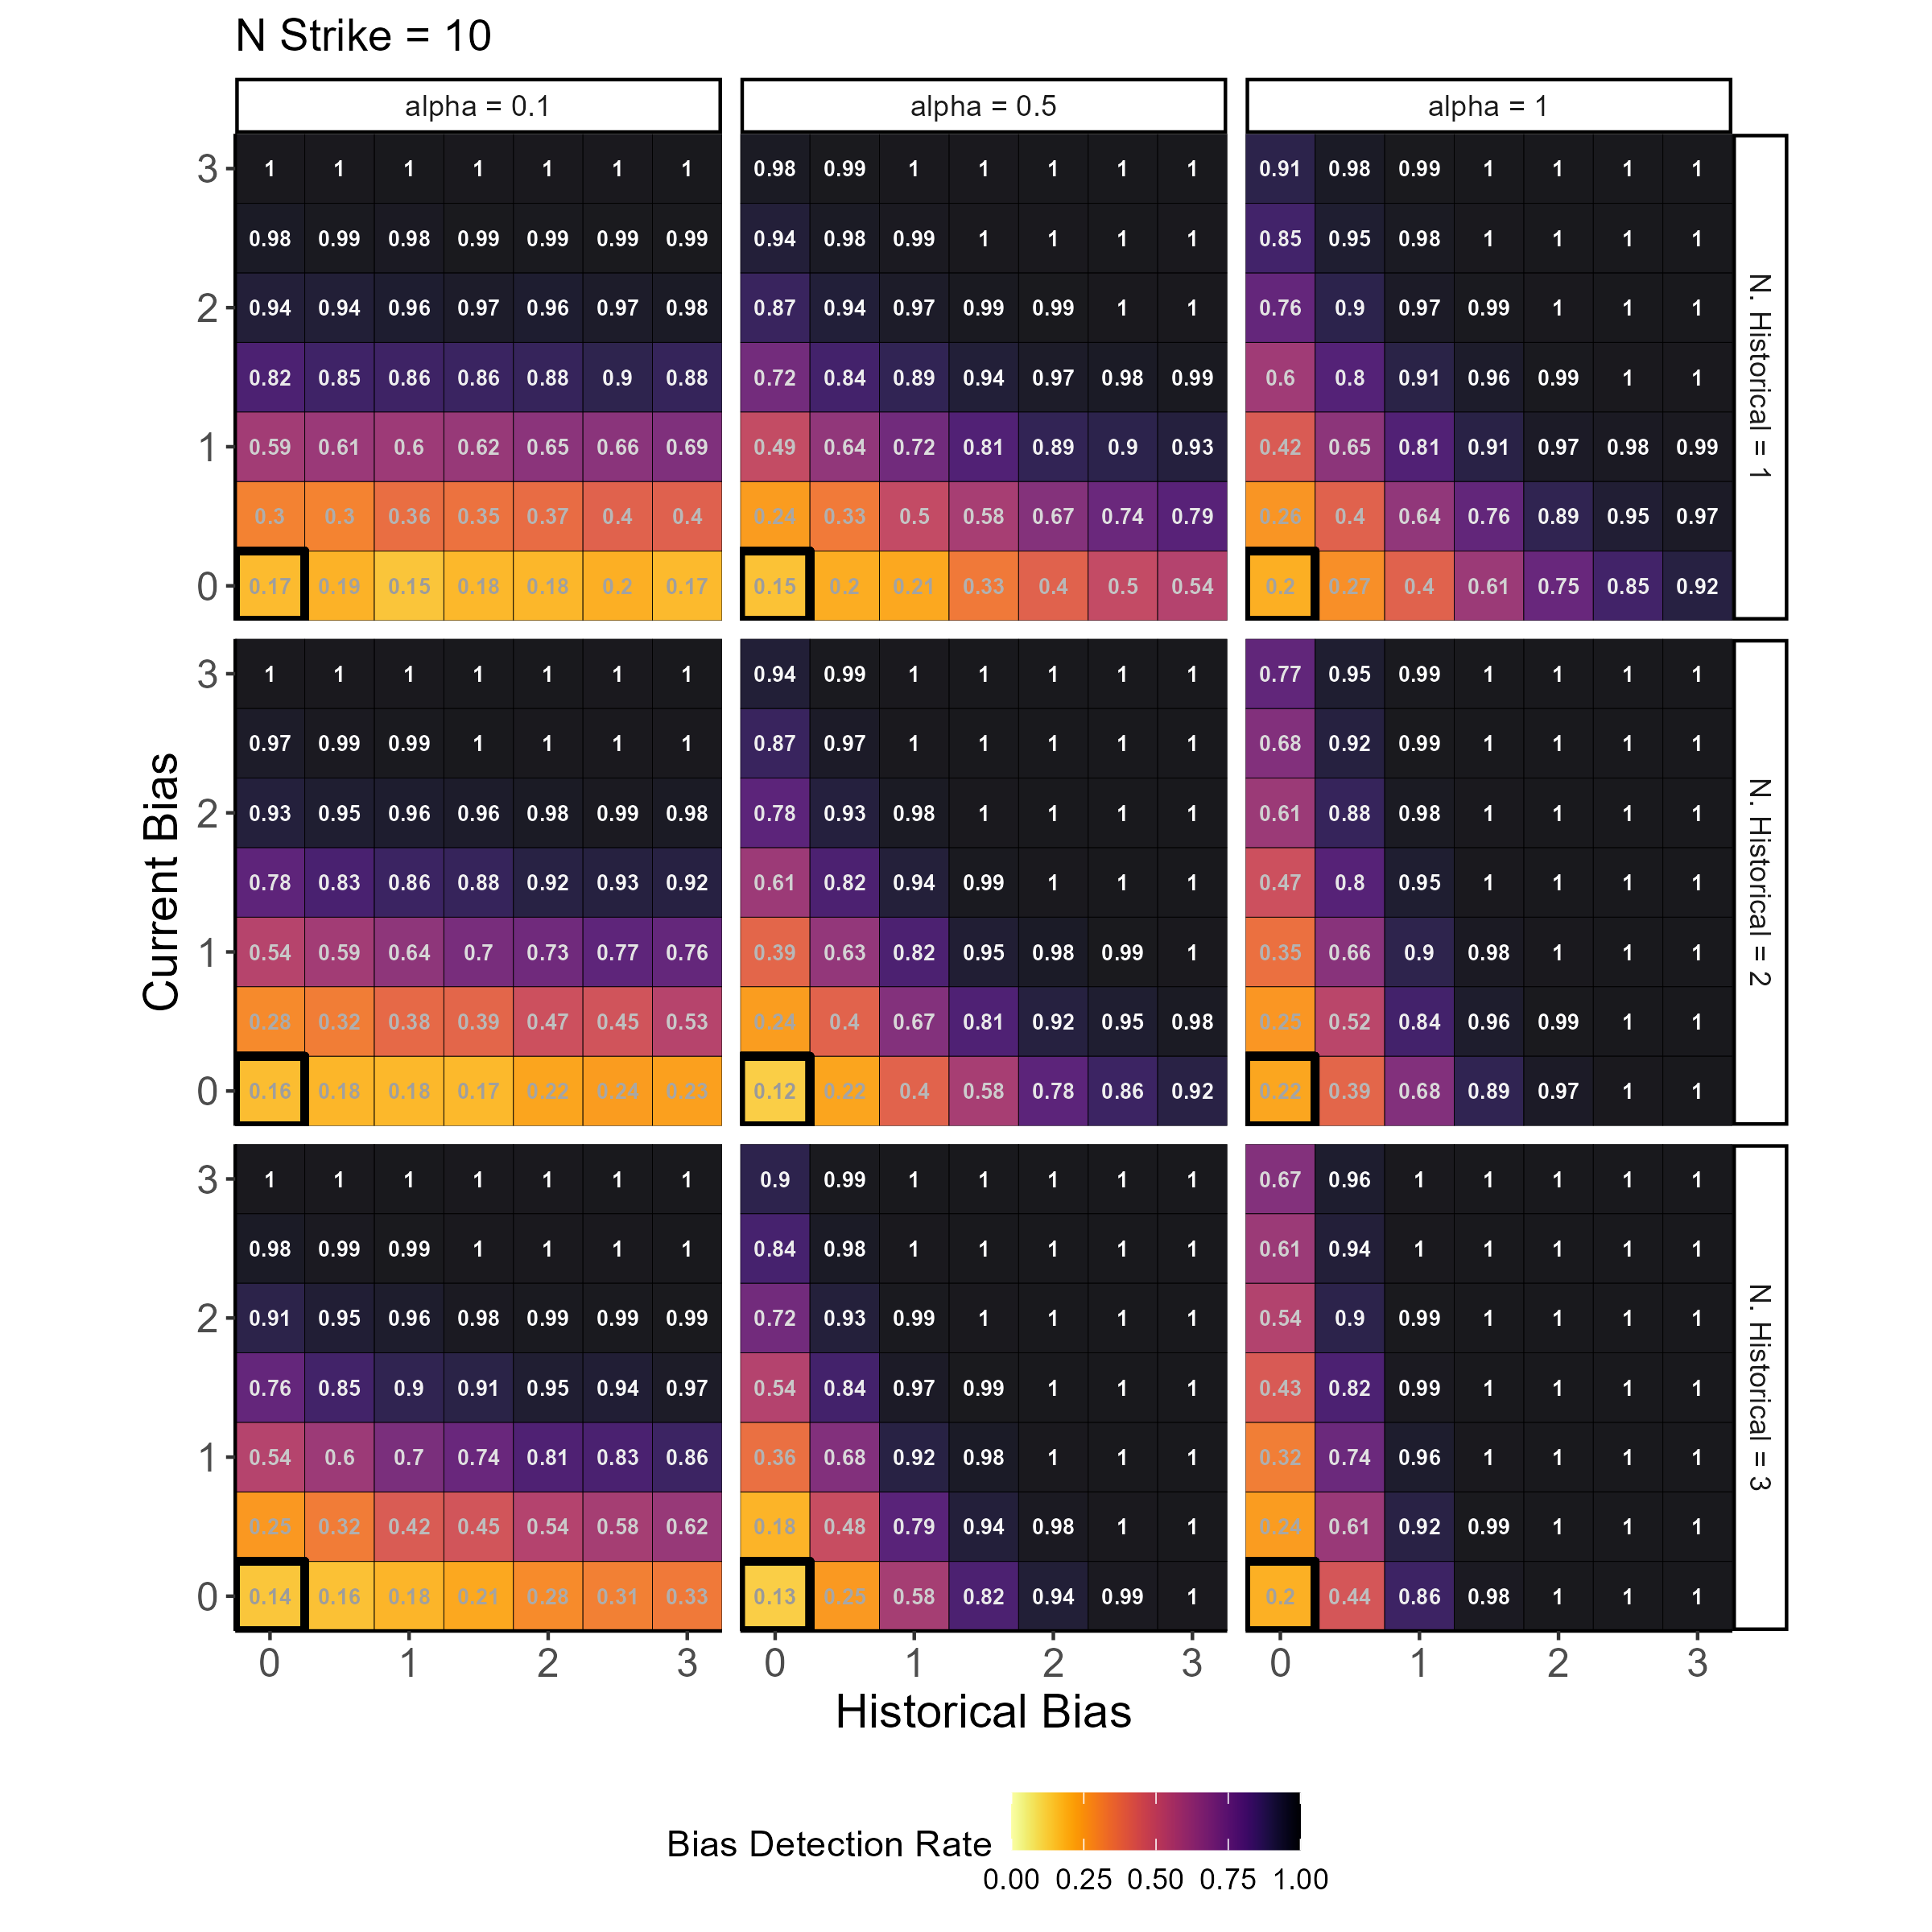
\includegraphics[width=0.95\linewidth]{../figures/pp10_80CI} 

}

\caption{Bias Detection Rates (80 pct credible interval, 10 strikes scenario)}\label{fig:figbd8010}
\end{figure}

\begin{figure}

{\centering 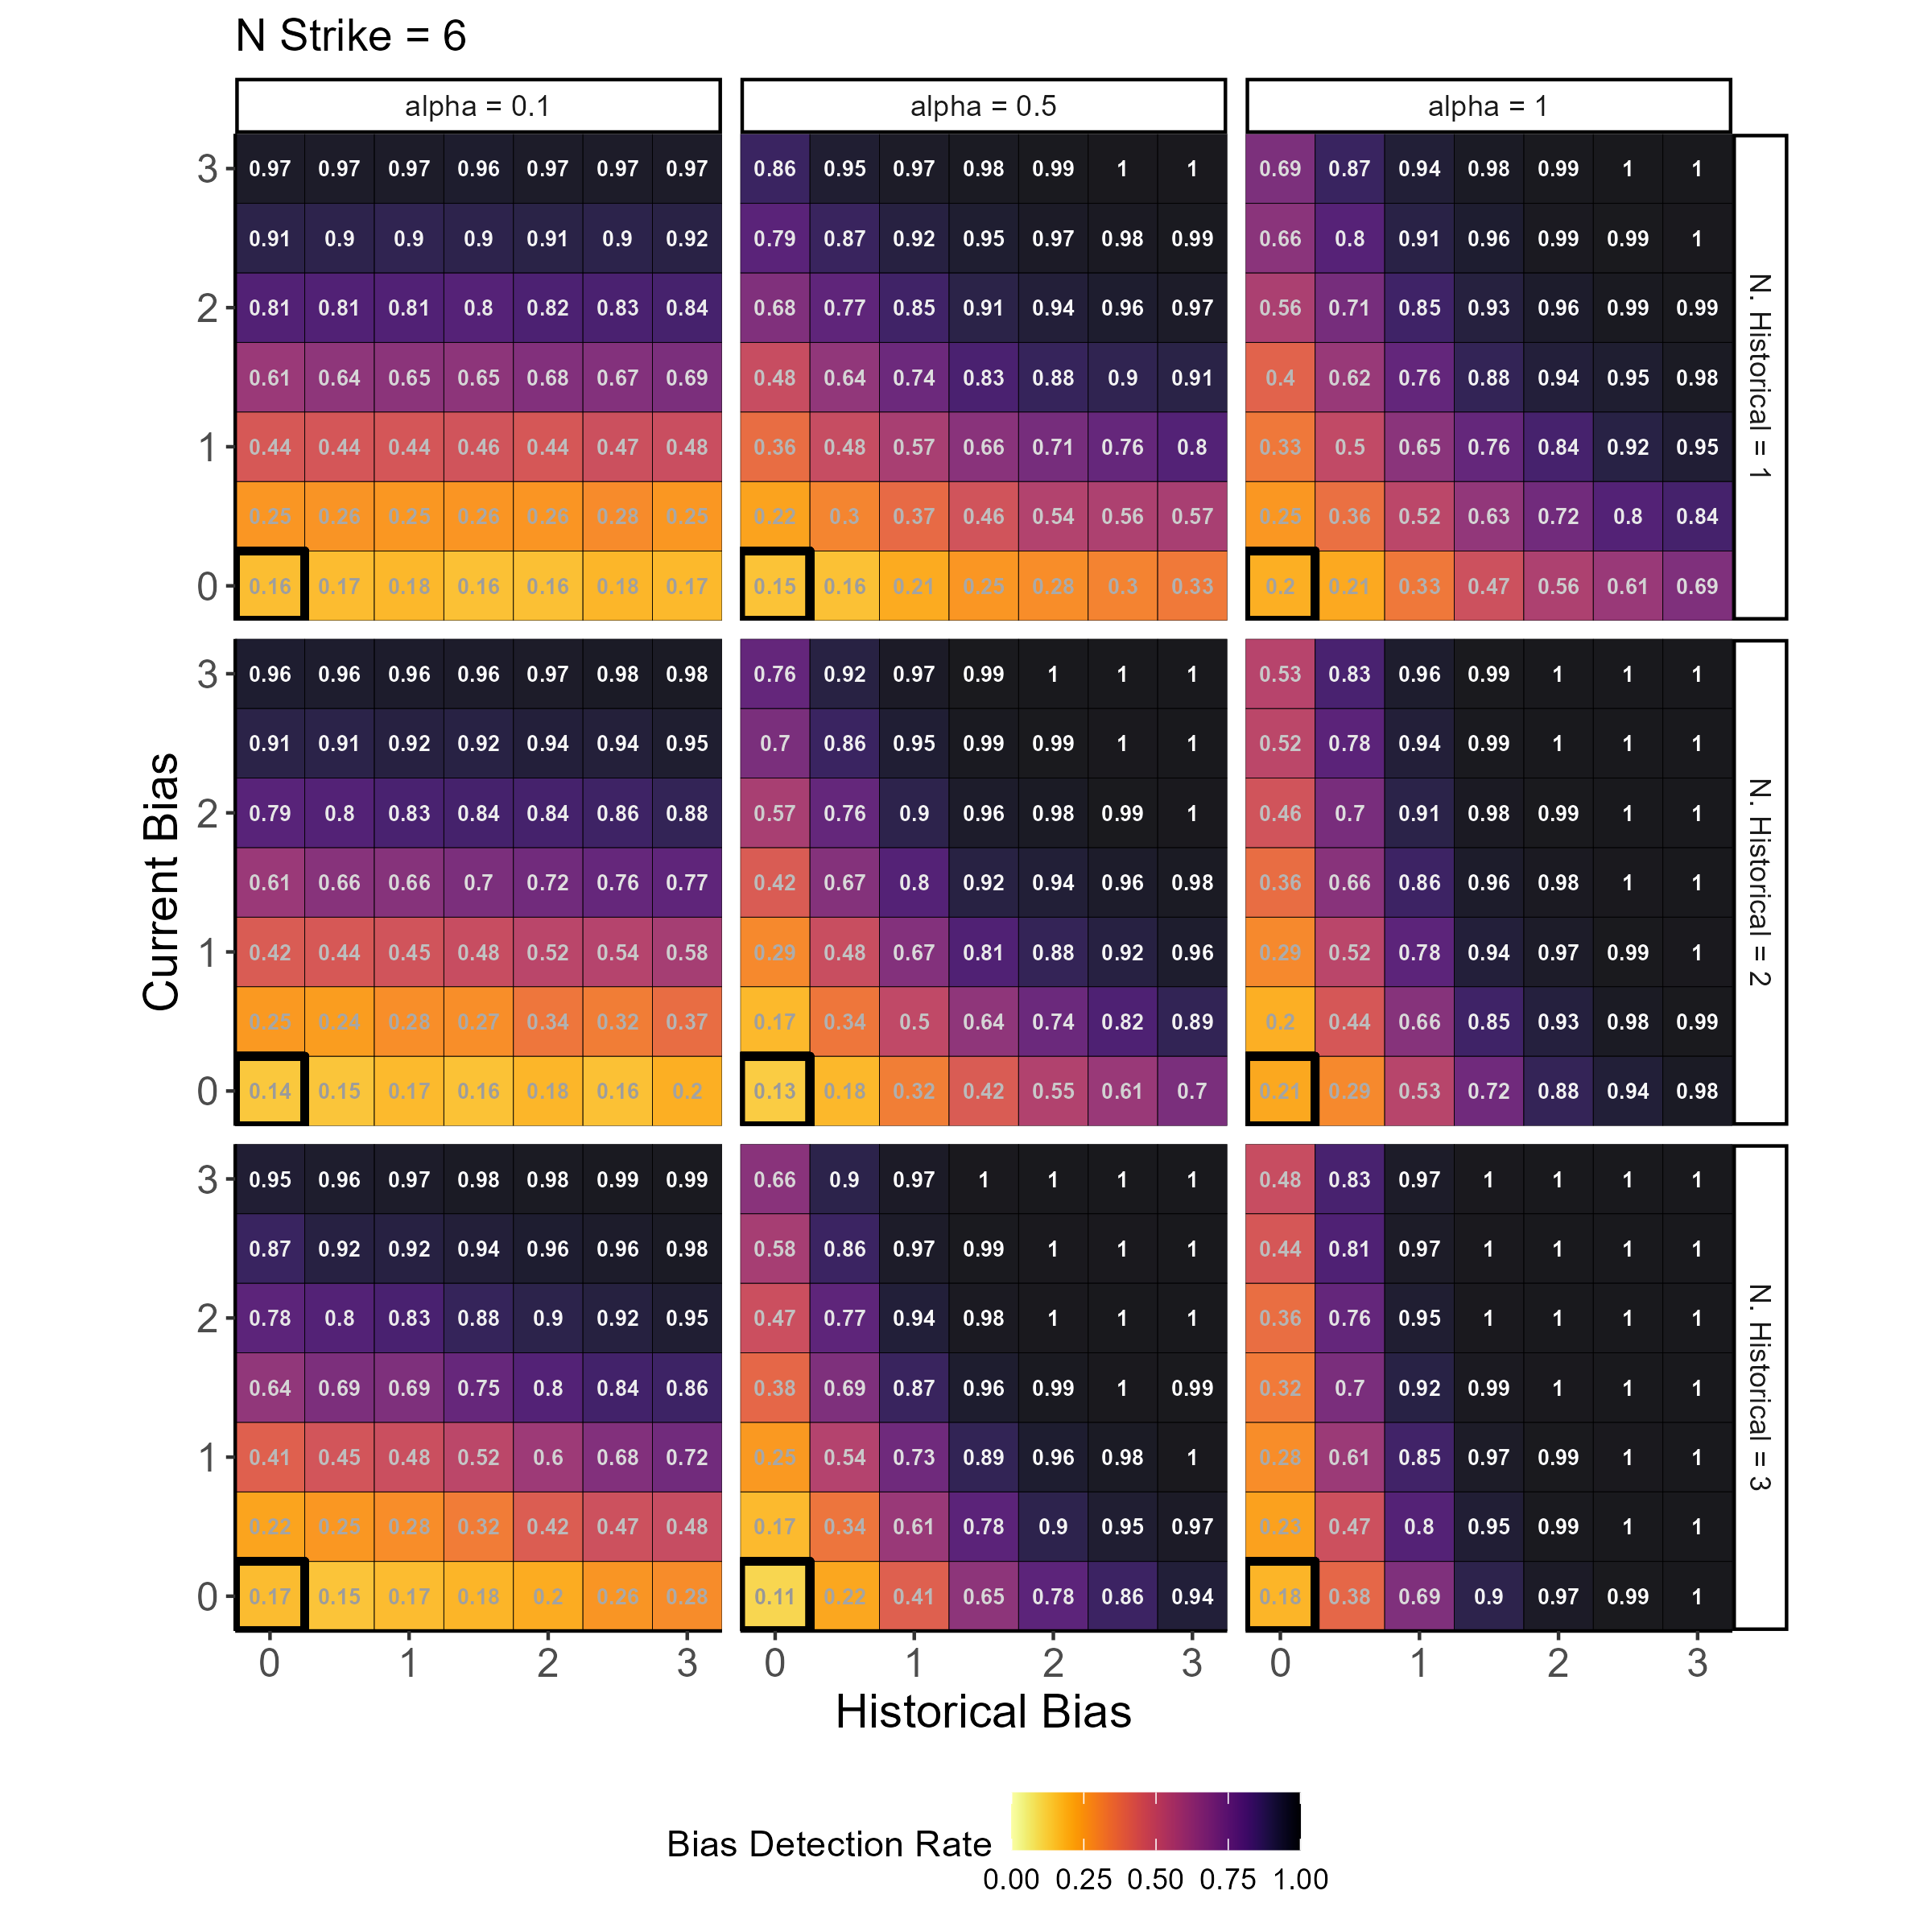
\includegraphics[width=0.95\linewidth]{../figures/pp6_80CI} 

}

\caption{Bias Detection Rates based on 80 pct credible interval for 6 strike scenario}\label{fig:figbd806}
\end{figure}

\hypertarget{prototype-software-application}{%
\subsection{Prototype Software Application}\label{prototype-software-application}}

\hypertarget{data-collection}{%
\subsubsection{Data Collection}\label{data-collection}}

To collect the historical strike data for the prototype software application, one of us filed a request with the U.S. District Court of Connecticut based on 28 U.S.C. \(\S\) 1868. Thereafter, we received copies of certain jury-selection records associated with twenty-nine criminal cases in that court during this period. These included strike sheets that indicated the identification number of prospective jurors who were struck by peremptory challenge, the order in which they were struck, and which side (prosecutor or defense) struck which juror. Such records also included a tally of answers to juror questionnaires that asked each prospective juror to report their race and gender.

These records, however, often did not indicate the identity of the attorneys exercising the strikes. While the standard forms included a signature line for the attorney, many were left blank or filled with illegible signatures. Accordingly, we turned to the publicly-available docket sheets for each case for the names of the lawyers who appeared in the case on behalf of the prosecution (the United States Attorney's office) or the criminal defendant(s) on the date(s) of jury selection. Where only a single attorney represented a party during jury selection, it was easy to attribute the pattern of strikes to that attorney. Where multiple lawyers appeared for one side, we attributed to each of them that side's pattern of peremptory challenges in that case. In such cases, neither the jury-selection documents nor the docket sheets indicated any hierarchy among multiple lawyers or any other basis to attribute strikes to only one attorney among them. After generating a dataset based on these documents, we kept only strikes where a criminal defendant was represented by an attorney. Finally, to de-identify this dataset, we excluded defendant names and substituted fictitious names for the attorneys using the charlatan package (Chamberlain and Voytovich 2020).

\hypertarget{additional-illustrations}{%
\subsubsection{Additional Illustrations}\label{additional-illustrations}}

Suppose the same scenario discussed in section 3.2 of the paper, except now the strike tally indicates the pattern of strikes by these attorneys against female prospective jurors. If so, we select ``gender'' as the cognizable class, and the density plots update accordingly (Figure \ref{fig:figapp3}(left)).

\begin{figure}
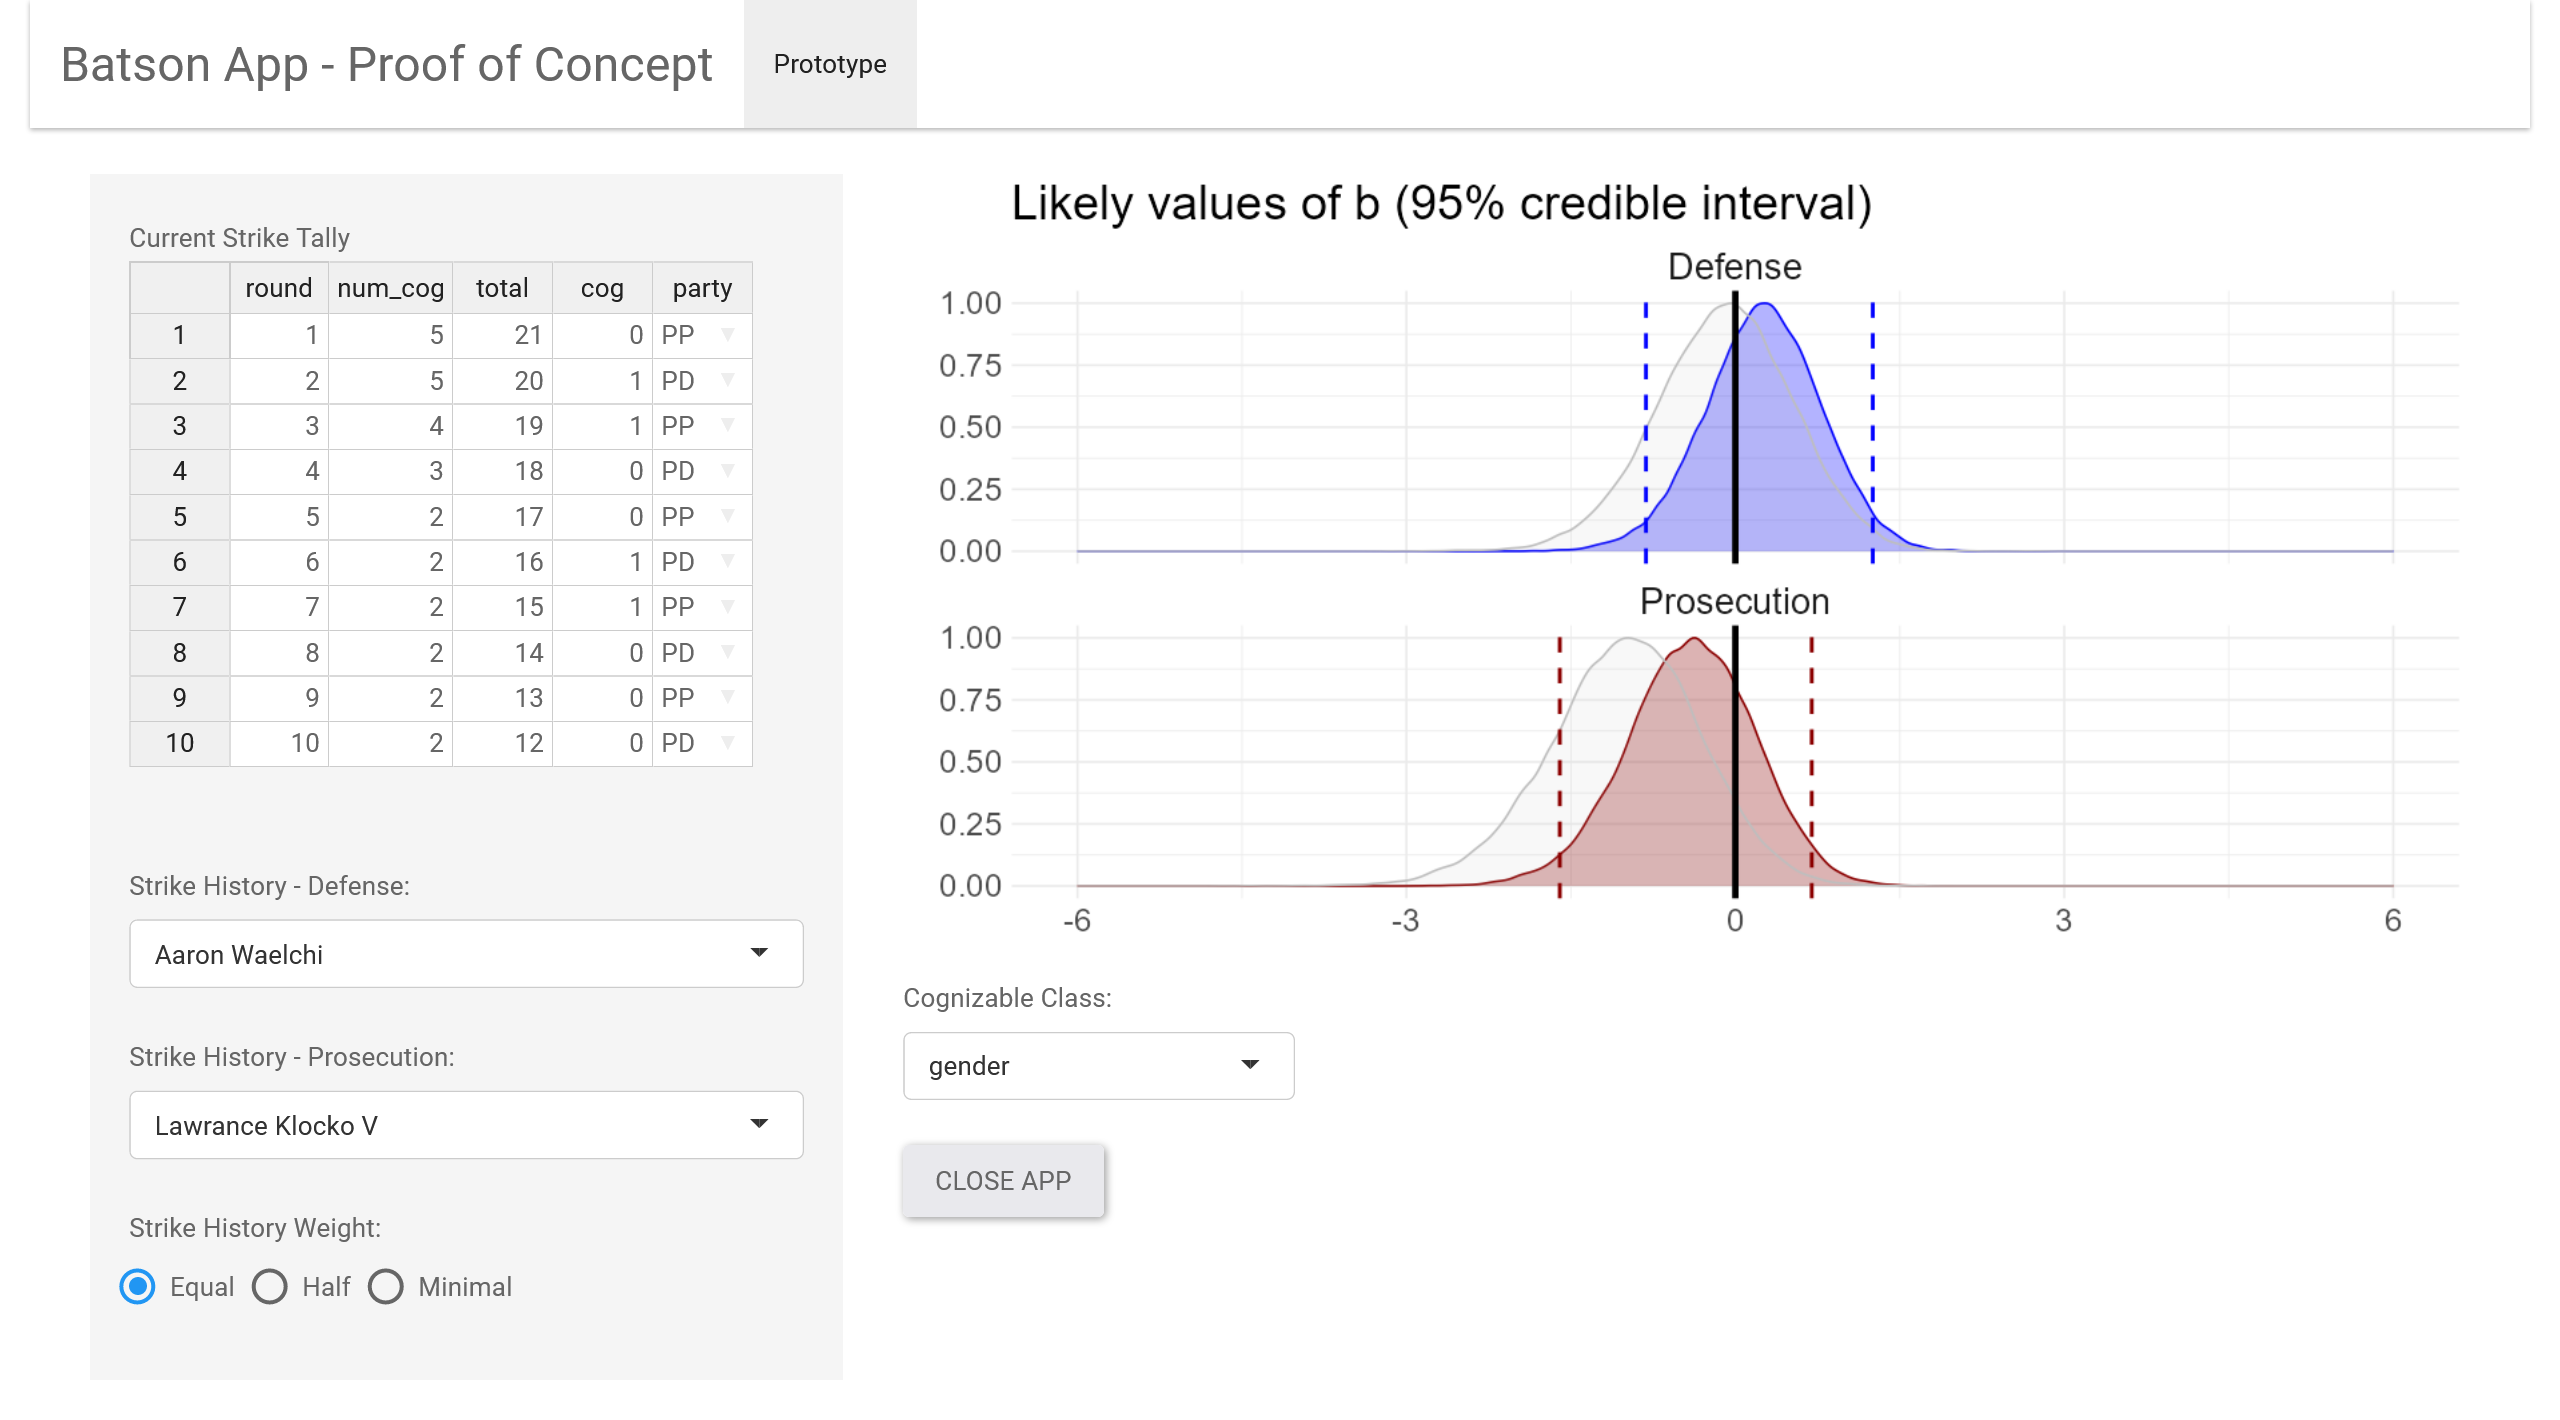
\includegraphics[width=0.5\linewidth]{../figures/batson_app_screenshots/batson_app_screenshot3} 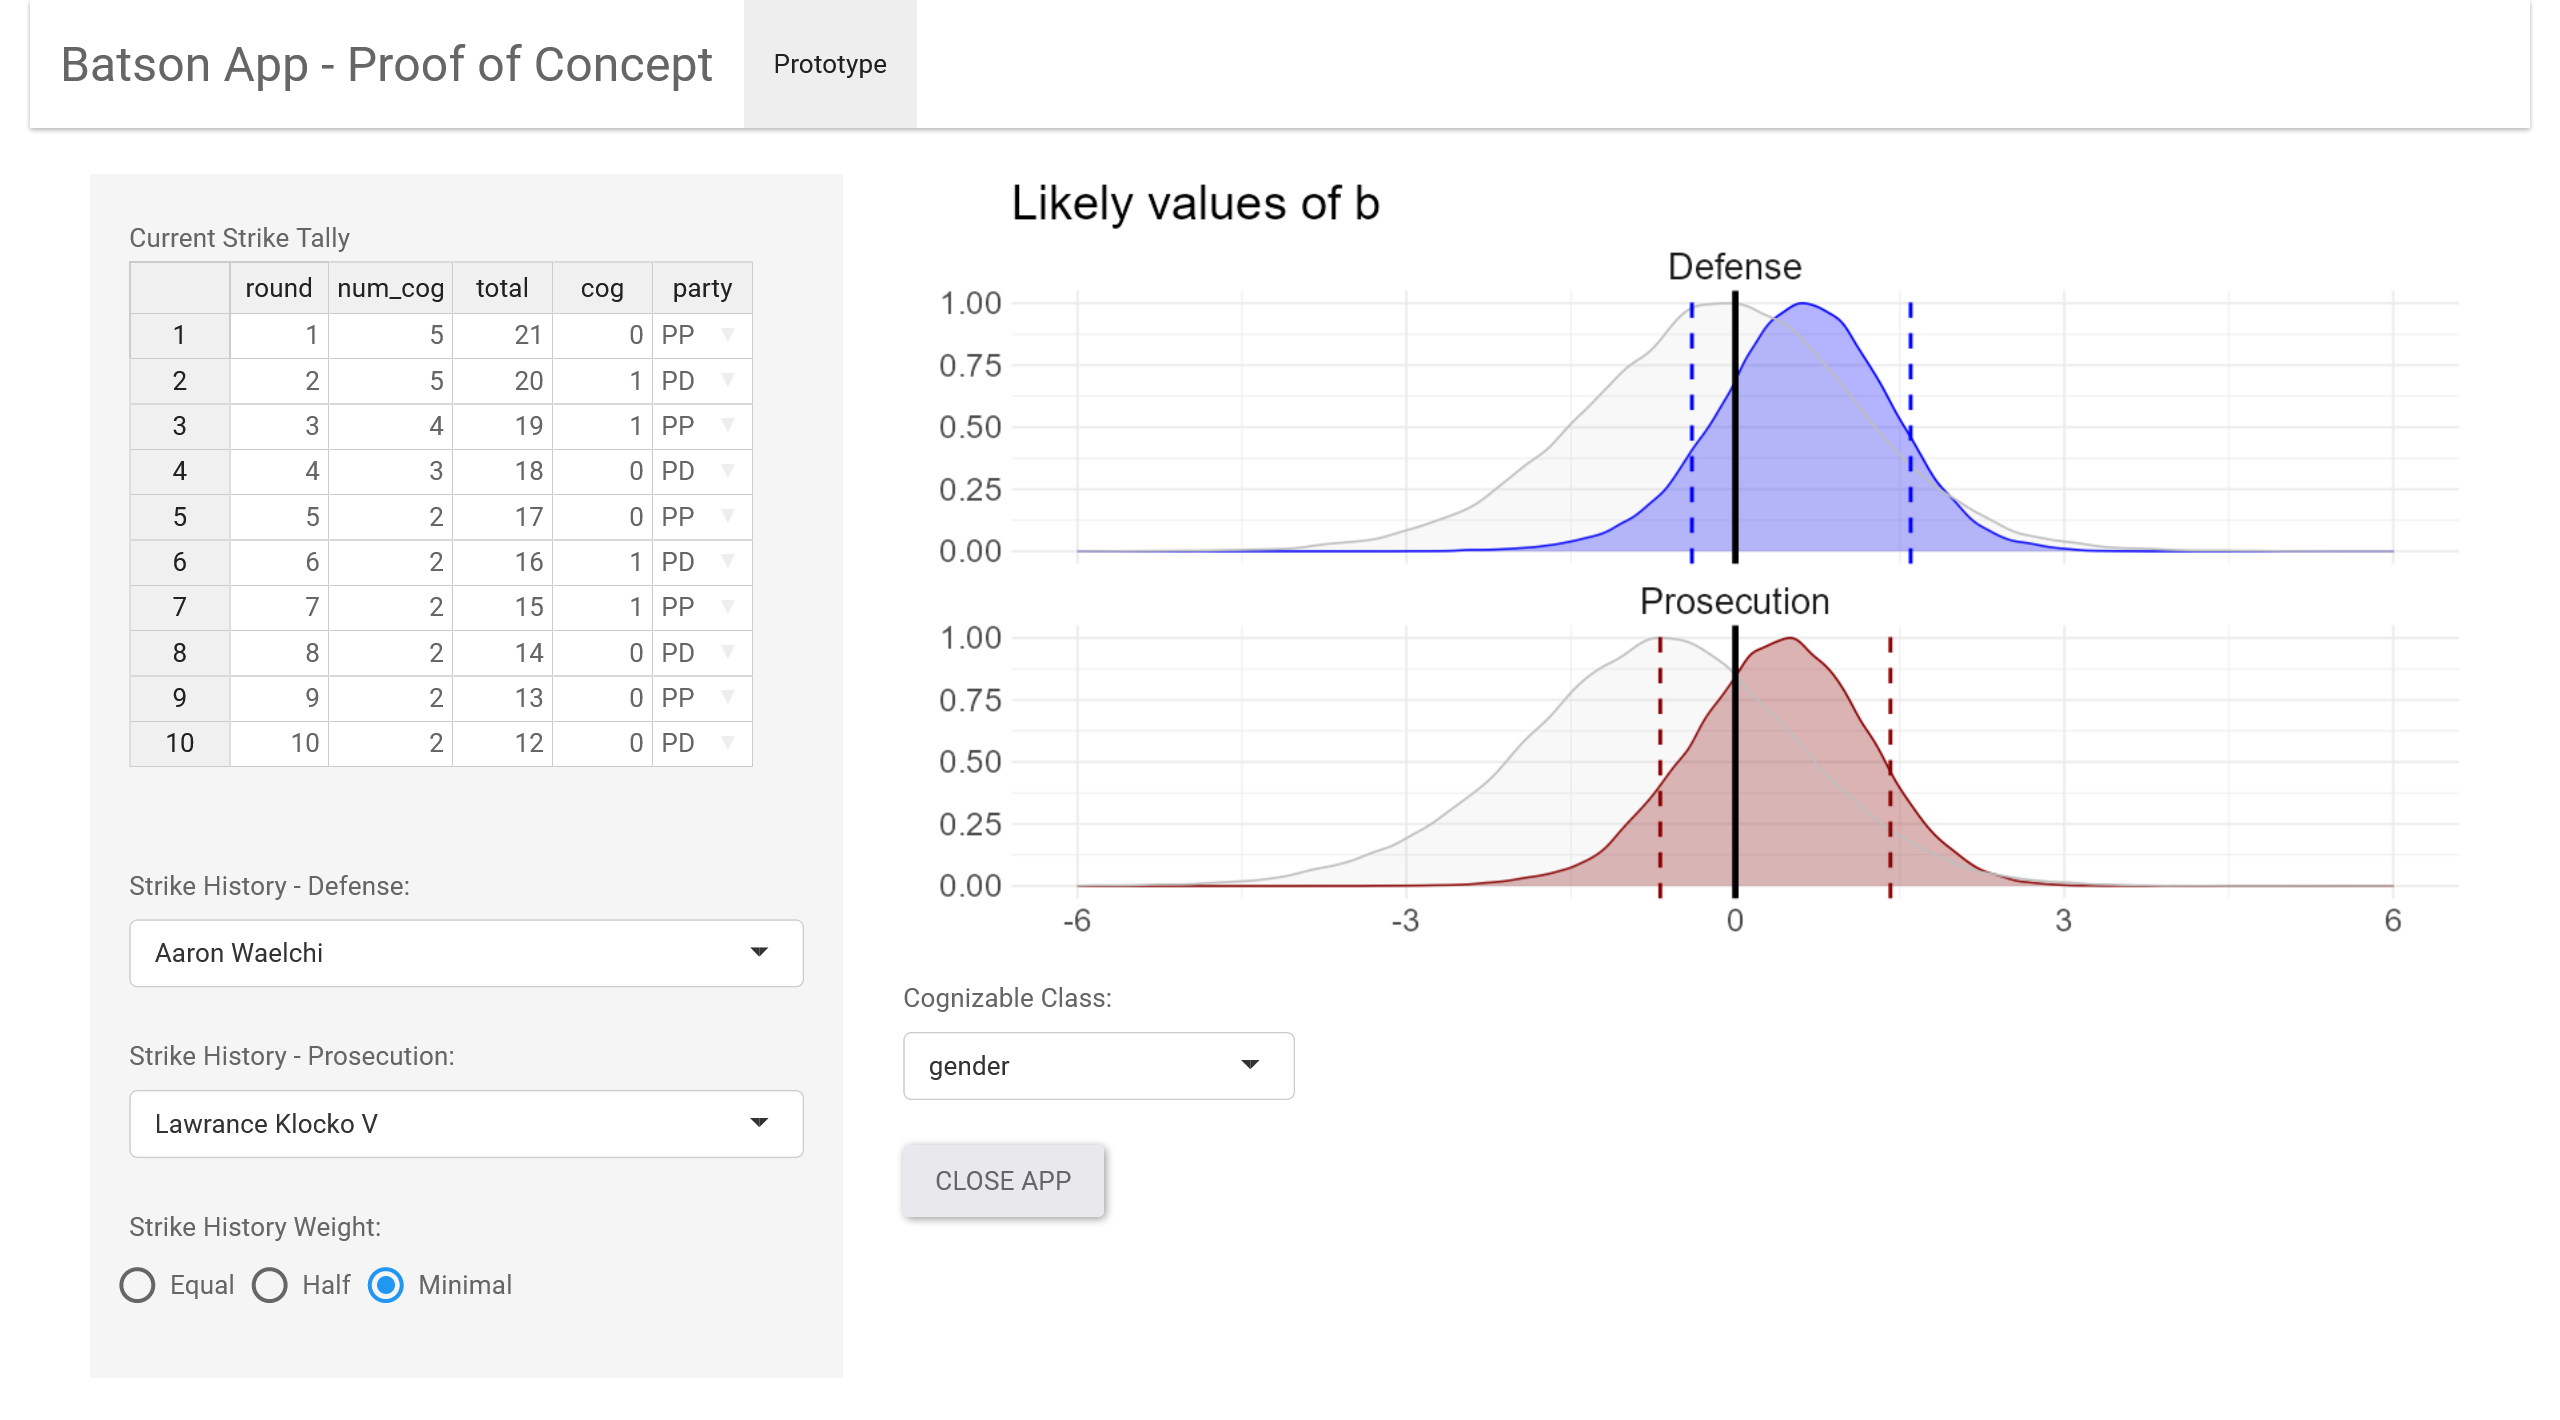
\includegraphics[width=0.5\linewidth]{../figures/batson_app_screenshots/batson_app_screenshot4} \caption{Screenshots of R-Shiny application show density plots for gender bias of prosecutor and defense attorney based on historical and current strike data. Vertical dotted lines depict 95 pct. credible interval.}\label{fig:figapp3}
\end{figure}

Here, most of the prosecutor's density curve of both prior and posterior are to the left of zero, indicating the possible bias against male jurors. However, because the 95\% credible interval includes zero, inferring such bias from the strike data alone is unjustified. Finally, if we assign minimal weight to the historical strike data (\(a = 0.1\)), the density plot updates accordingly (Figure \ref{fig:figapp3}(right)). Both the prior and posterior density become flatter and the credible interval plainly includes zero.

\hypertarget{refs}{}
\begin{CSLReferences}{1}{0}
\leavevmode\vadjust pre{\hypertarget{ref-charlatan}{}}%
Chamberlain, Scott, and Kyle Voytovich. 2020. \emph{Charlatan: Make Fake Data}. \url{https://CRAN.R-project.org/package=charlatan}.

\end{CSLReferences}



\end{document}
